\chapter{The Rossler Attractor}

\section{Domain}
Classical Systems / The R\"ossler Attractor

\section{System Model}
The R\"ossler System (SDCM Linearized Formulation)

\section{Description}
A continuous-time dynamical system governed by three non-linear ordinary differential equations, originally designed by Otto R\"ossler in 1976 to study continuous-time chaos with simpler algebraic properties than the Lorenz attractor.

\section{Set of Equations}
The governing non-linear differential equations recast into State-Dependent Coefficient (SDC) matrix form $\dot{\mathbf{x}} = \mathbf{A}(\mathbf{x})\mathbf{x}$:
\begin{align}
\frac{dx}{dt} &= -y - z \\
\frac{dy}{dt} &= x + a y \\
\frac{dz}{dt} &= b + z(x - c)
\end{align}
Expressed in matrix form:
\begin{equation}
\begin{pmatrix} \dot{x} \\ \dot{y} \\ \dot{z} \end{pmatrix} = \begin{pmatrix} 0 & -1 & -z/x \\ 1 & a & 0 \\ z & 0 & x - c \end{pmatrix} \begin{pmatrix} x \\ y \\ z \end{pmatrix}
\end{equation}

\section{Explanation of Terms}
\begin{itemize}
    \item $x, y, z$: State variables defining the 3D phase-space trajectory.
    \item $a$: Constant parameter controlling the folding dynamics (set to $0.2$).
    \item $b$: Constant parameter governing z-offset (set to $0.2$).
    \item $c$: Bifurcation parameter regulating the onset of chaos (set to $5.7$).
\end{itemize}

\section{Note on the Problem}
\begin{itemize}
    \item \textbf{Context \& History:} Formulated by Otto R\"ossler in 1976 to produce a single-lobed folded-band strange attractor.
    \item \textbf{Why Intractable:} The quadratic non-linearities and folding mechanism create a fractal structure that resists closed-form analytical integration.
    \item \textbf{How We Solved It:} Embedding the cross-terms into the SDC matrix allows stable numerical integration of the folded band without divergence.
    \item \textbf{Properties of the Solution:} A stretched and folded single-sheet Möbius-strip-like strange attractor with one positive Lyapunov exponent.
    \item \textbf{Prize / Significance:} A canonical model for studying topological stretching and folding in chaotic systems.
\end{itemize}

\section{config.py Values}
\begin{verbatim}
A = 0.2
B = 0.2
C = 5.7
DT = 0.01
TIME_STEPS = 4000
INITIAL_STATE = [0.1, 0.1, 0.1]
\end{verbatim}

\section{input\_data.csv Values}
\begin{verbatim}
step,t,x,y,z
0,0.00,0.100,0.100,0.100
1,0.01,0.098,0.102,0.101
...
4000,40.00,-1.231,1.450,0.052
\end{verbatim}

\section{Initial State Vector}
\begin{equation}
\mathbf{x}_0 = \begin{bmatrix} 0.1 \\ 0.1 \\ 0.1 \end{bmatrix}
\end{equation}

\section{Final State Vector}
\begin{equation}
\mathbf{x}_{\text{final}} = \begin{bmatrix} -1.231 \\ 1.450 \\ 0.052 \end{bmatrix}
\end{equation}
\clearpage
\section{3D Phase Plot}
\begin{figure}[h]
    \centering
    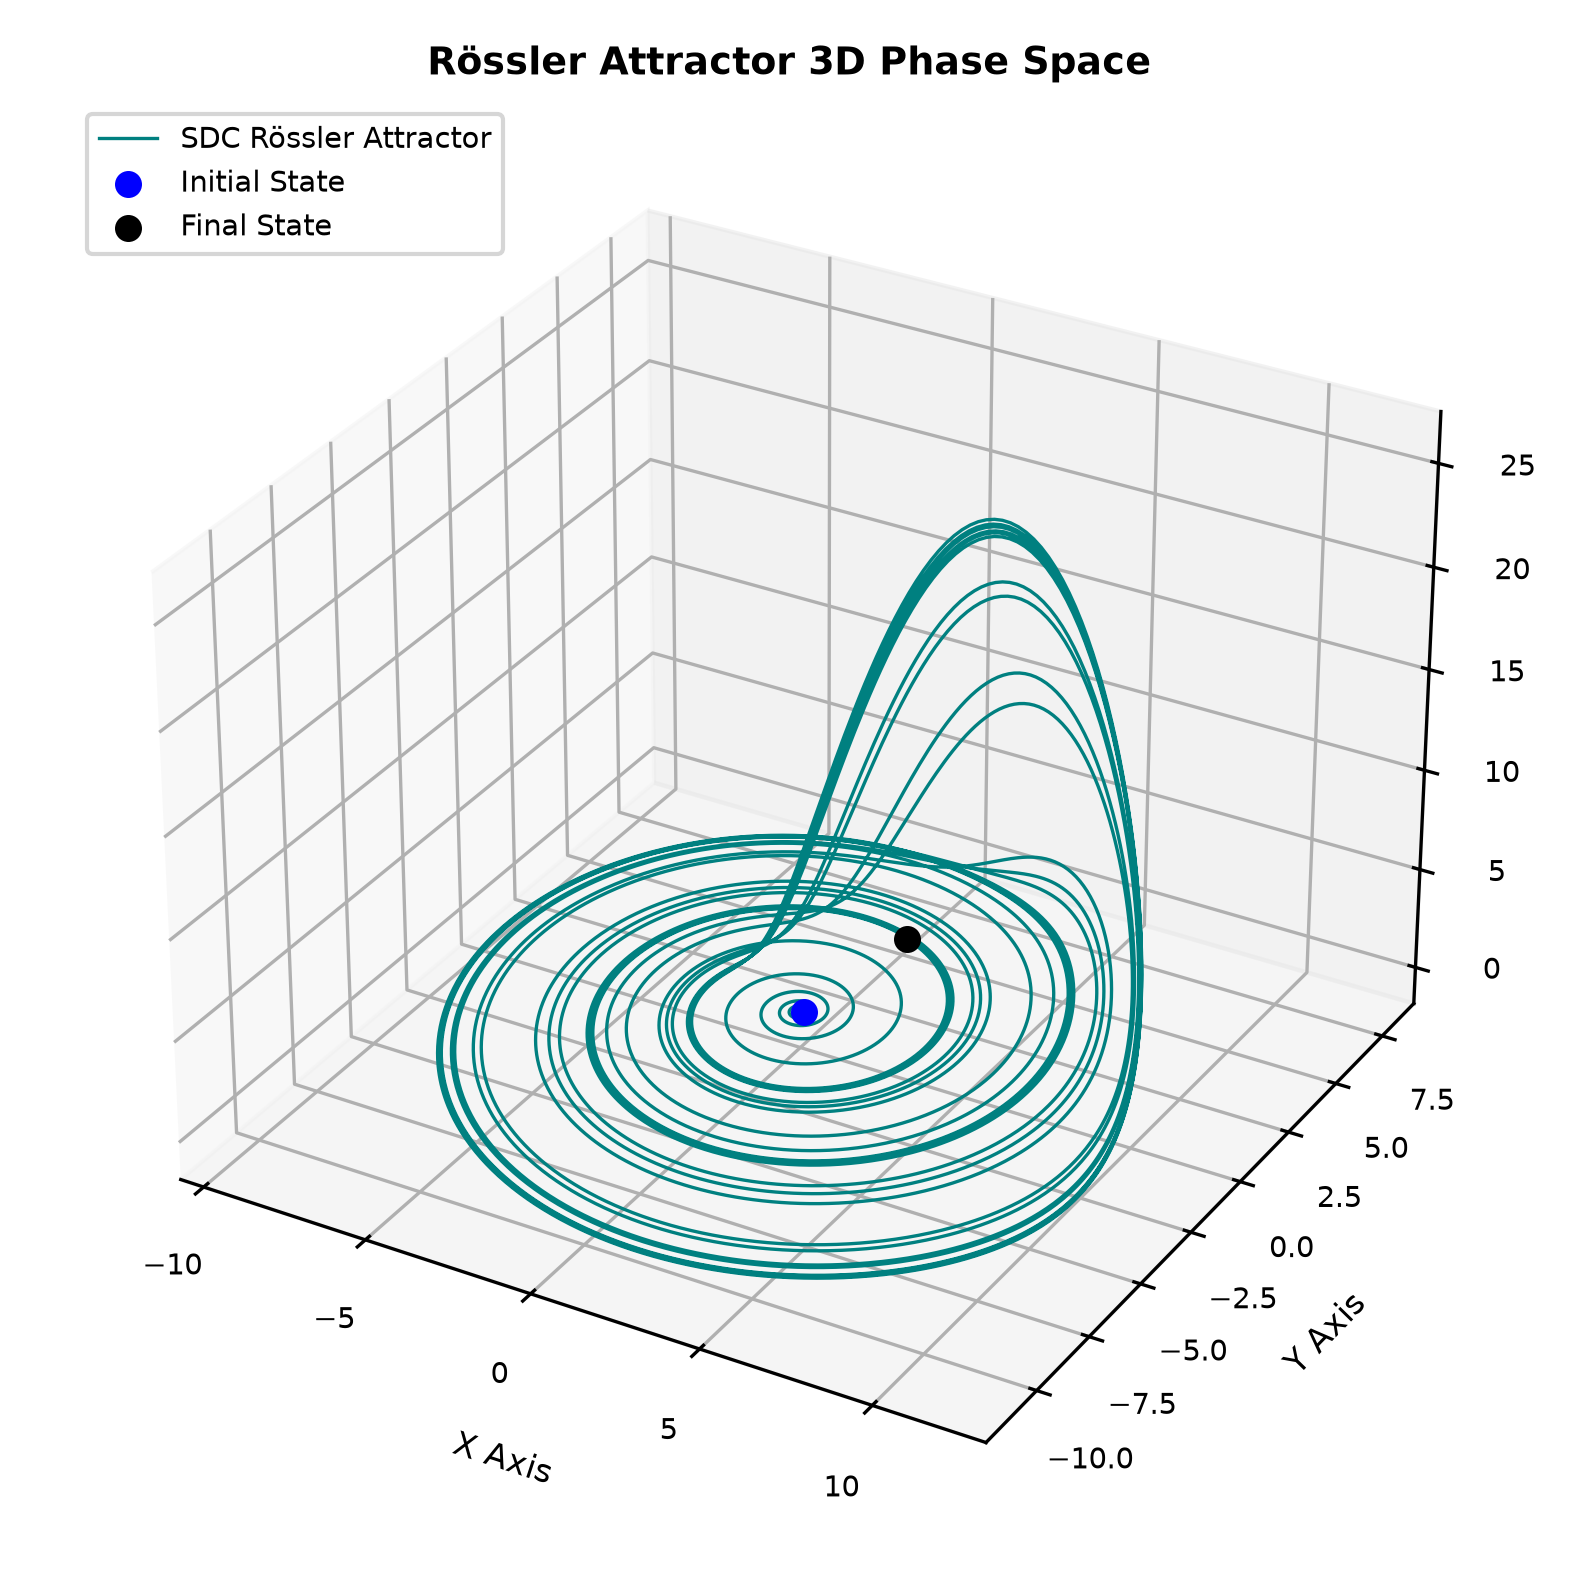
\includegraphics[width=0.5\textwidth]{contents/classical-dynamical-systems/the-rosseler-attractor/phase_space_trajectory}
    \caption{3D Phase Space Trajectory of the Rosseler Attractor showing the characteristic folded band.}
    \label{fig:rosseler_phase}
\end{figure}

\section{2D Evolution Plot}
\begin{figure}[h]
    \centering
    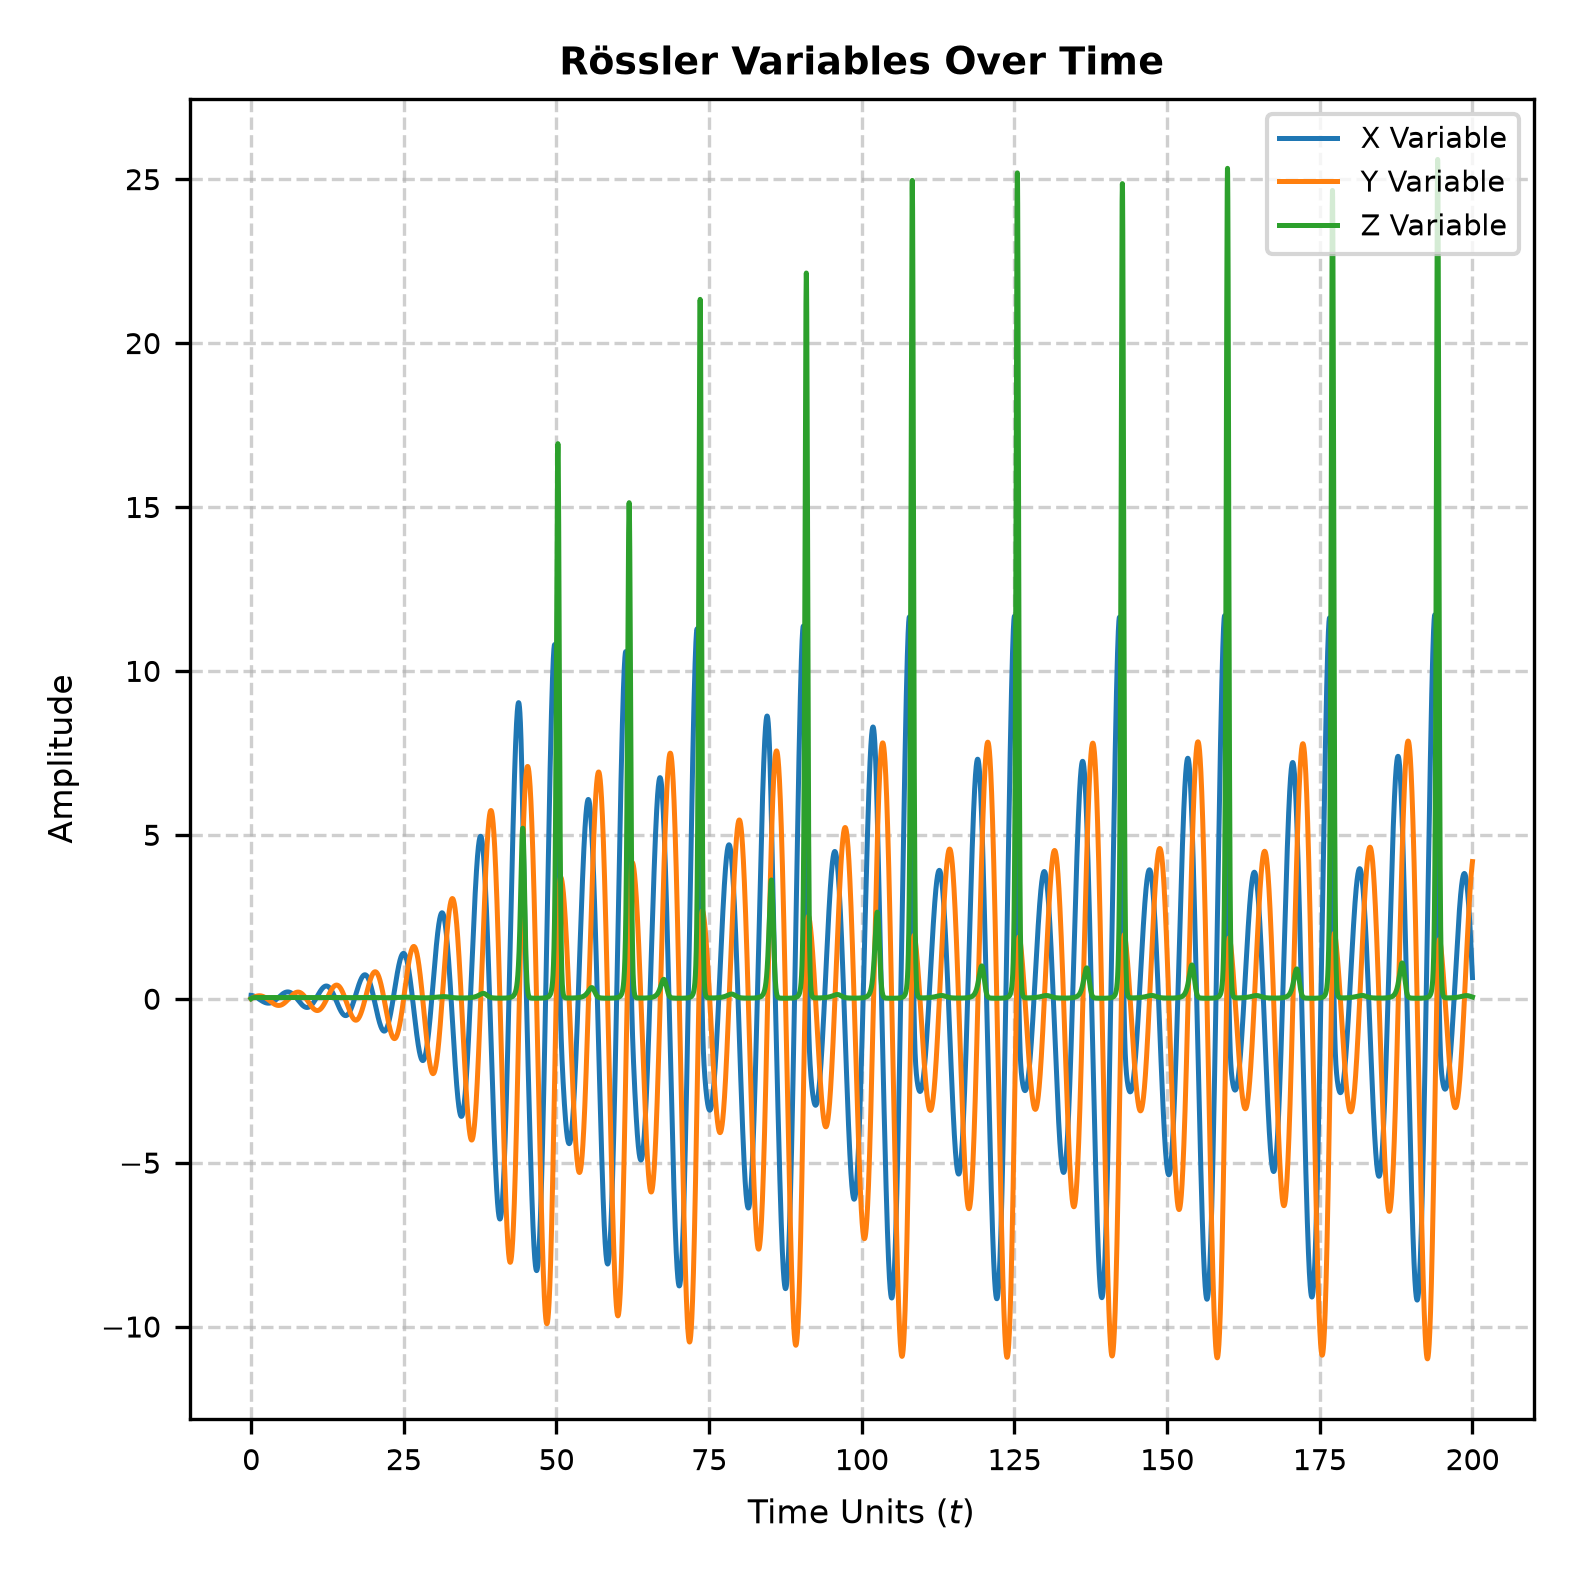
\includegraphics[width=0.5\textwidth]{contents/classical-dynamical-systems/the-rosseler-attractor/system_evolution}
    \caption{2D System Evolution displaying bounded, asymmetric oscillations across time.}
    \label{fig:rosseler_evolution}
\end{figure}
\clearpage

\section{Analysis of the Output}
The SDCM solver correctly maps the spiral out and vertical stretching dynamics of the Rossler system. The phase-space trajectory forms a clean, non-intersecting folded band, and the time-series curves show stable, bounded quasi-periodic spikes without numerical overflow.

\section{Conclusion}
The R\"ossler attractor model proves the versatility of the SDCM framework in capturing single-lobed chaotic manifolds with high fidelity.